%!TEX TS-program = xelatex

% Этот шаблон документа разработан в 2014 году
% Данилом Фёдоровых (danil@fedorovykh.ru) 
% для использования в курсе 
% <<Документы и презентации в \LaTeX>>, записанном НИУ ВШЭ
% для Coursera.org: http://coursera.org/course/latex .
% Исходная версия шаблона --- 
% https://www.writelatex.com/coursera/latex/5.2.2

\documentclass[a4paper,12pt]{article}

%%% Работа с русским языком
\usepackage[english,russian]{babel}   %% загружает пакет многоязыковой вёрстки
\usepackage{fontspec}      %% подготавливает загрузку шрифтов Open Type, True Type и др.
\defaultfontfeatures{Ligatures={TeX},Renderer=Basic}  %% свойства шрифтов по умолчанию
\setmainfont[Ligatures={TeX,Historic}]{Times New Roman} %% задаёт основной шрифт документа
\setsansfont{Comic Sans MS}                    %% задаёт шрифт без засечек
\setmonofont{Courier New}
\usepackage{indentfirst}
\frenchspacing

\renewcommand{\epsilon}{\ensuremath{\varepsilon}}
\renewcommand{\phi}{\ensuremath{\varphi}}
\renewcommand{\kappa}{\ensuremath{\varkappa}}
\renewcommand{\le}{\ensuremath{\leqslant}}
\renewcommand{\leq}{\ensuremath{\leqslant}}
\renewcommand{\ge}{\ensuremath{\geqslant}}
\renewcommand{\geq}{\ensuremath{\geqslant}}
\renewcommand{\emptyset}{\varnothing}

%%% Дополнительная работа с математикой
\usepackage{amsmath,amsfonts,amssymb,amsthm,mathtools} % AMS
\usepackage{icomma} % "Умная" запятая: $0,2$ --- число, $0, 2$ --- перечисление

%% Номера формул
%\mathtoolsset{showonlyrefs=true} % Показывать номера только у тех формул, на которые есть \eqref{} в тексте.
%\usepackage{leqno} % Нумерация формул слева

%% Свои команды
\DeclareMathOperator{\sgn}{\mathop{sgn}}

%% Перенос знаков в формулах (по Львовскому)
\newcommand*{\hm}[1]{#1\nobreak\discretionary{}
	{\hbox{$\mathsurround=0pt #1$}}{}}

%%% Работа с картинками
\usepackage{graphicx}  % Для вставки рисунков
\graphicspath{{images/}{images2/}}  % папки с картинками
\setlength\fboxsep{3pt} % Отступ рамки \fbox{} от рисунка
\setlength\fboxrule{1pt} % Толщина линий рамки \fbox{}
\usepackage{wrapfig} % Обтекание рисунков текстом

%%% Работа с таблицами
\usepackage{array,tabularx,tabulary,booktabs} % Дополнительная работа с таблицами
\usepackage{longtable}  % Длинные таблицы
\usepackage{multirow} % Слияние строк в таблице

%%% Теоремы
\theoremstyle{plain} % Это стиль по умолчанию, его можно не переопределять.
\newtheorem{theorem}{Теорема}[section]
\newtheorem{proposition}[theorem]{Утверждение}

\theoremstyle{definition} % "Определение"
\newtheorem{corollary}{Следствие}[theorem]
\newtheorem{problem}{Задача}[section]

\theoremstyle{remark} % "Примечание"
\newtheorem*{nonum}{Решение}

%%% Программирование
\usepackage{etoolbox} % логические операторы


%%% Страница
\usepackage{extsizes} % Возможность сделать 14-й шрифт
\usepackage{geometry} % Простой способ задавать поля
\geometry{top=5mm}
\geometry{bottom=15mm}
\geometry{left=5mm}
\geometry{right=5mm}
%
%\usepackage{fancyhdr} % Колонтитулы
% 	\pagestyle{fancy}
%\renewcommand{\headrulewidth}{0pt}  % Толщина линейки, отчеркивающей верхний колонтитул
% 	\lfoot{Нижний левый}
% 	\rfoot{Нижний правый}
% 	\rhead{Верхний правый}
% 	\chead{Верхний в центре}
% 	\lhead{Верхний левый}
%	\cfoot{Нижний в центре} % По умолчанию здесь номер страницы

\usepackage{setspace} % Интерлиньяж
%\onehalfspacing % Интерлиньяж 1.5
%\doublespacing % Интерлиньяж 2
%\singlespacing % Интерлиньяж 1

\usepackage{lastpage} % Узнать, сколько всего страниц в документе.

\usepackage{soul} % Модификаторы начертания

\usepackage{hyperref}
\usepackage[usenames,dvipsnames,svgnames,table,rgb]{xcolor}
\hypersetup{				% Гиперссылки
	unicode=true,           % русские буквы в раздела PDF
	pdftitle={Заголовок},   % Заголовок
	pdfauthor={Автор},      % Автор
	pdfsubject={Тема},      % Тема
	pdfcreator={Создатель}, % Создатель
	pdfproducer={Производитель}, % Производитель
	pdfkeywords={keyword1} {key2} {key3}, % Ключевые слова
	colorlinks=true,       	% false: ссылки в рамках; true: цветные ссылки
	linkcolor=red,          % внутренние ссылки
	citecolor=black,        % на библиографию
	filecolor=magenta,      % на файлы
	urlcolor=cyan           % на URL
}

\usepackage{csquotes} % Еще инструменты для ссылок

%\usepackage[style=authoryear,maxcitenames=2,backend=biber,sorting=nty]{biblatex}

\usepackage{multicol} % Несколько колонок

\usepackage{tikz} % Работа с графикой
\usepackage{pgfplots}
\usepackage{pgfplotstable}

\author{Батарин Егор}
\title{Описание лавинного эффекта.}
\date{}
\begin{document} % конец преамбулы, начало документа
	
	\maketitle
По определению, хэш-функция обладает свойсвом лавинного эффекта, если при изменении одного бита входной последовательности меняется в среднем половина битов выходной последовательности. Цель проекта - проверить, выполняется ли данный критерий для алгоритма Keccak.

Для этого в проекте генерируются пары строк, отличающихся на один бит - входные последовательности. Далее сравнимаются выходные последовательности и считается количество измененных бит. По полученным данным строятся графики, на оси абсцисс которых отображен процент измененных бит, а ось ординат выражает меру количества таких строк. Стоит ожидать, что максимум графика будет достигаться при $50\%$.

Ниже приведена таблица, которая в зависимости от размера хэша и количества проведенных раундов показывает среднее значение модифицированных бит в процентах.

% Please add the following required packages to your document preamble:
% \usepackage{multirow}
\begin{table}[h!]
	\centering
	\begin{tabular}{|l|lllllll|}
		\hline
		\multirow{2}{*}{\begin{tabular}[c]{@{}l@{}}Размер\\ хэша\\\end{tabular}} & \multicolumn{7}{l|}{Число раундов}                                                                                                                                                         \\ \cline{2-8} 
		& \multicolumn{1}{l|}{1}      & \multicolumn{1}{l|}{2}      & \multicolumn{1}{l|}{3}      & \multicolumn{1}{l|}{4}      & \multicolumn{1}{l|}{8}      & \multicolumn{1}{l|}{12}     & 24     \\ \hline
		224                                                                           & \multicolumn{1}{l|}{37.995} & \multicolumn{1}{l|}{48.504} & \multicolumn{1}{l|}{50.041} & \multicolumn{1}{l|}{50.151} & \multicolumn{1}{l|}{50.196} & \multicolumn{1}{l|}{49.882} & 49.882 \\ \hline
		256                                                                           & \multicolumn{1}{l|}{36.716} & \multicolumn{1}{l|}{48.32}  & \multicolumn{1}{l|}{49.991} & \multicolumn{1}{l|}{49.875} & \multicolumn{1}{l|}{50.067} & \multicolumn{1}{l|}{50.102} & 50.045 \\ \hline
		384                                                                           & \multicolumn{1}{l|}{37.689} & \multicolumn{1}{l|}{48.609} & \multicolumn{1}{l|}{50.03}  & \multicolumn{1}{l|}{49.949} & \multicolumn{1}{l|}{50.092} & \multicolumn{1}{l|}{49.997} & 50.003 \\ \hline
		512                                                                           & \multicolumn{1}{l|}{40.136} & \multicolumn{1}{l|}{49.256} & \multicolumn{1}{l|}{50.072} & \multicolumn{1}{l|}{49.996} & \multicolumn{1}{l|}{49.979} & \multicolumn{1}{l|}{49.999} & 49.981 \\ \hline
	\end{tabular}
\end{table}

Как видим, уже начиная с числа раундов, равным 3, лавинный эффект проявляется в полной мере.

По графикам также можно сделать два качественных заключения по распределению доли модифицированных бит. Во-первых, начиная с третьего раунда, распределение очень хорошо аппроксимируется нормальным, как видно из картинки ниже.

\begin{figure}[ht!]
	\centering
	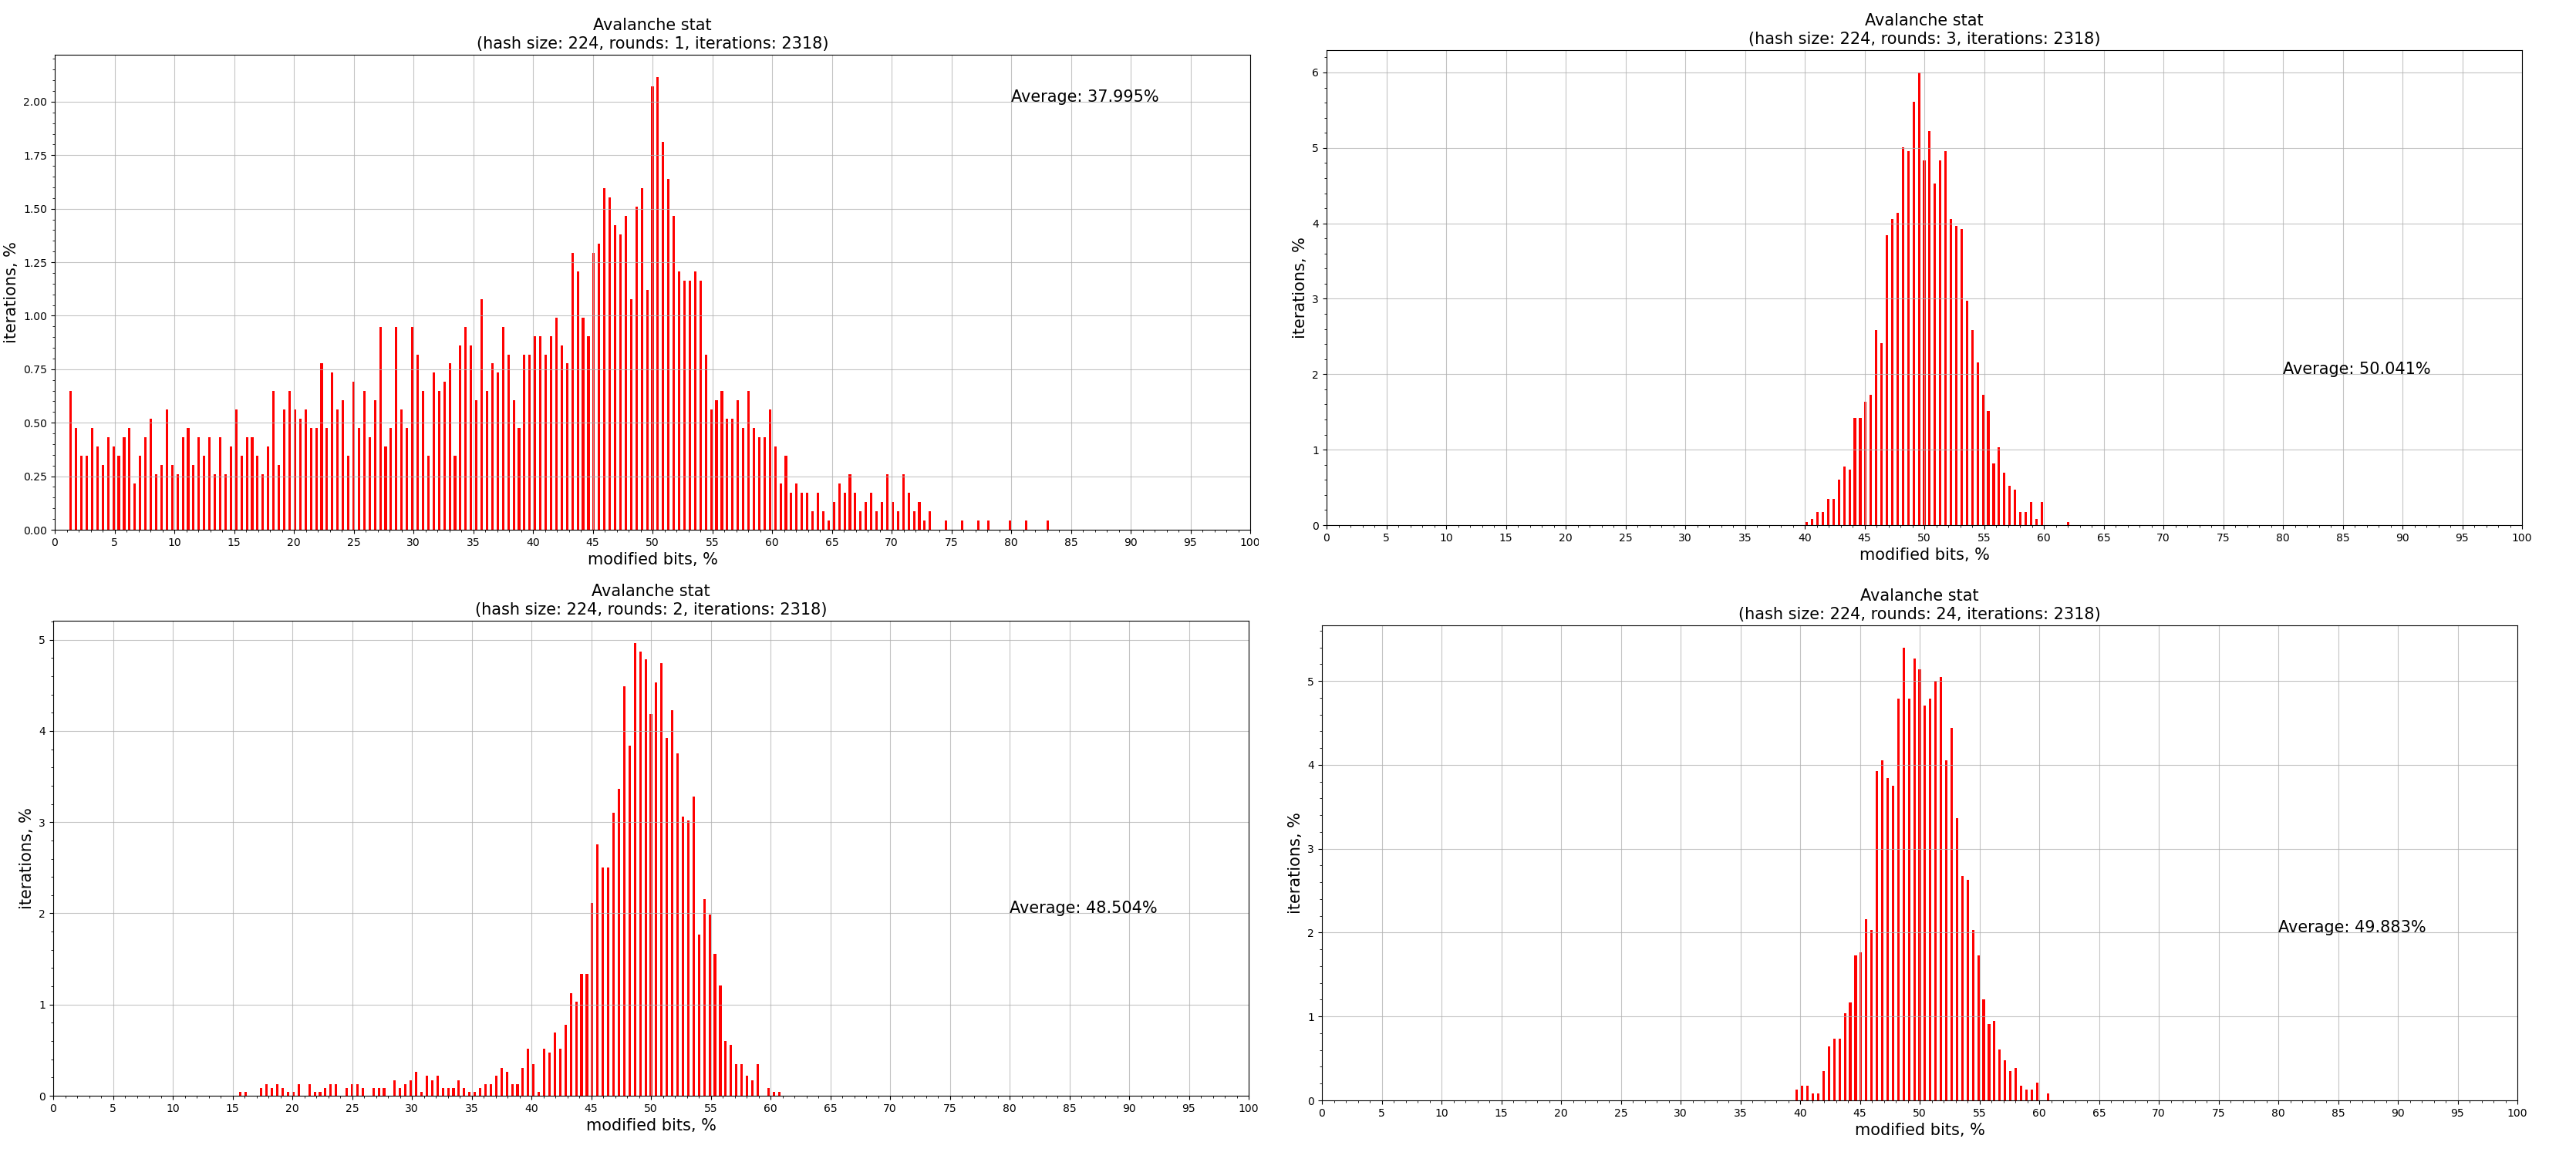
\includegraphics[width=165mm]{224-1_2_3_24.png}
	\caption{Хэш 224 бита с числом раундов 1, 2, 3 и 24}
\end{figure}

\newpage

Во-вторых, чем выше размер хэша, чем меньше дисперсия нормального распределенения. Ниже сравнение хэшей 224 и 512 бит с числом раундов, равным 24.

\begin{figure}[ht!]
	\centering
	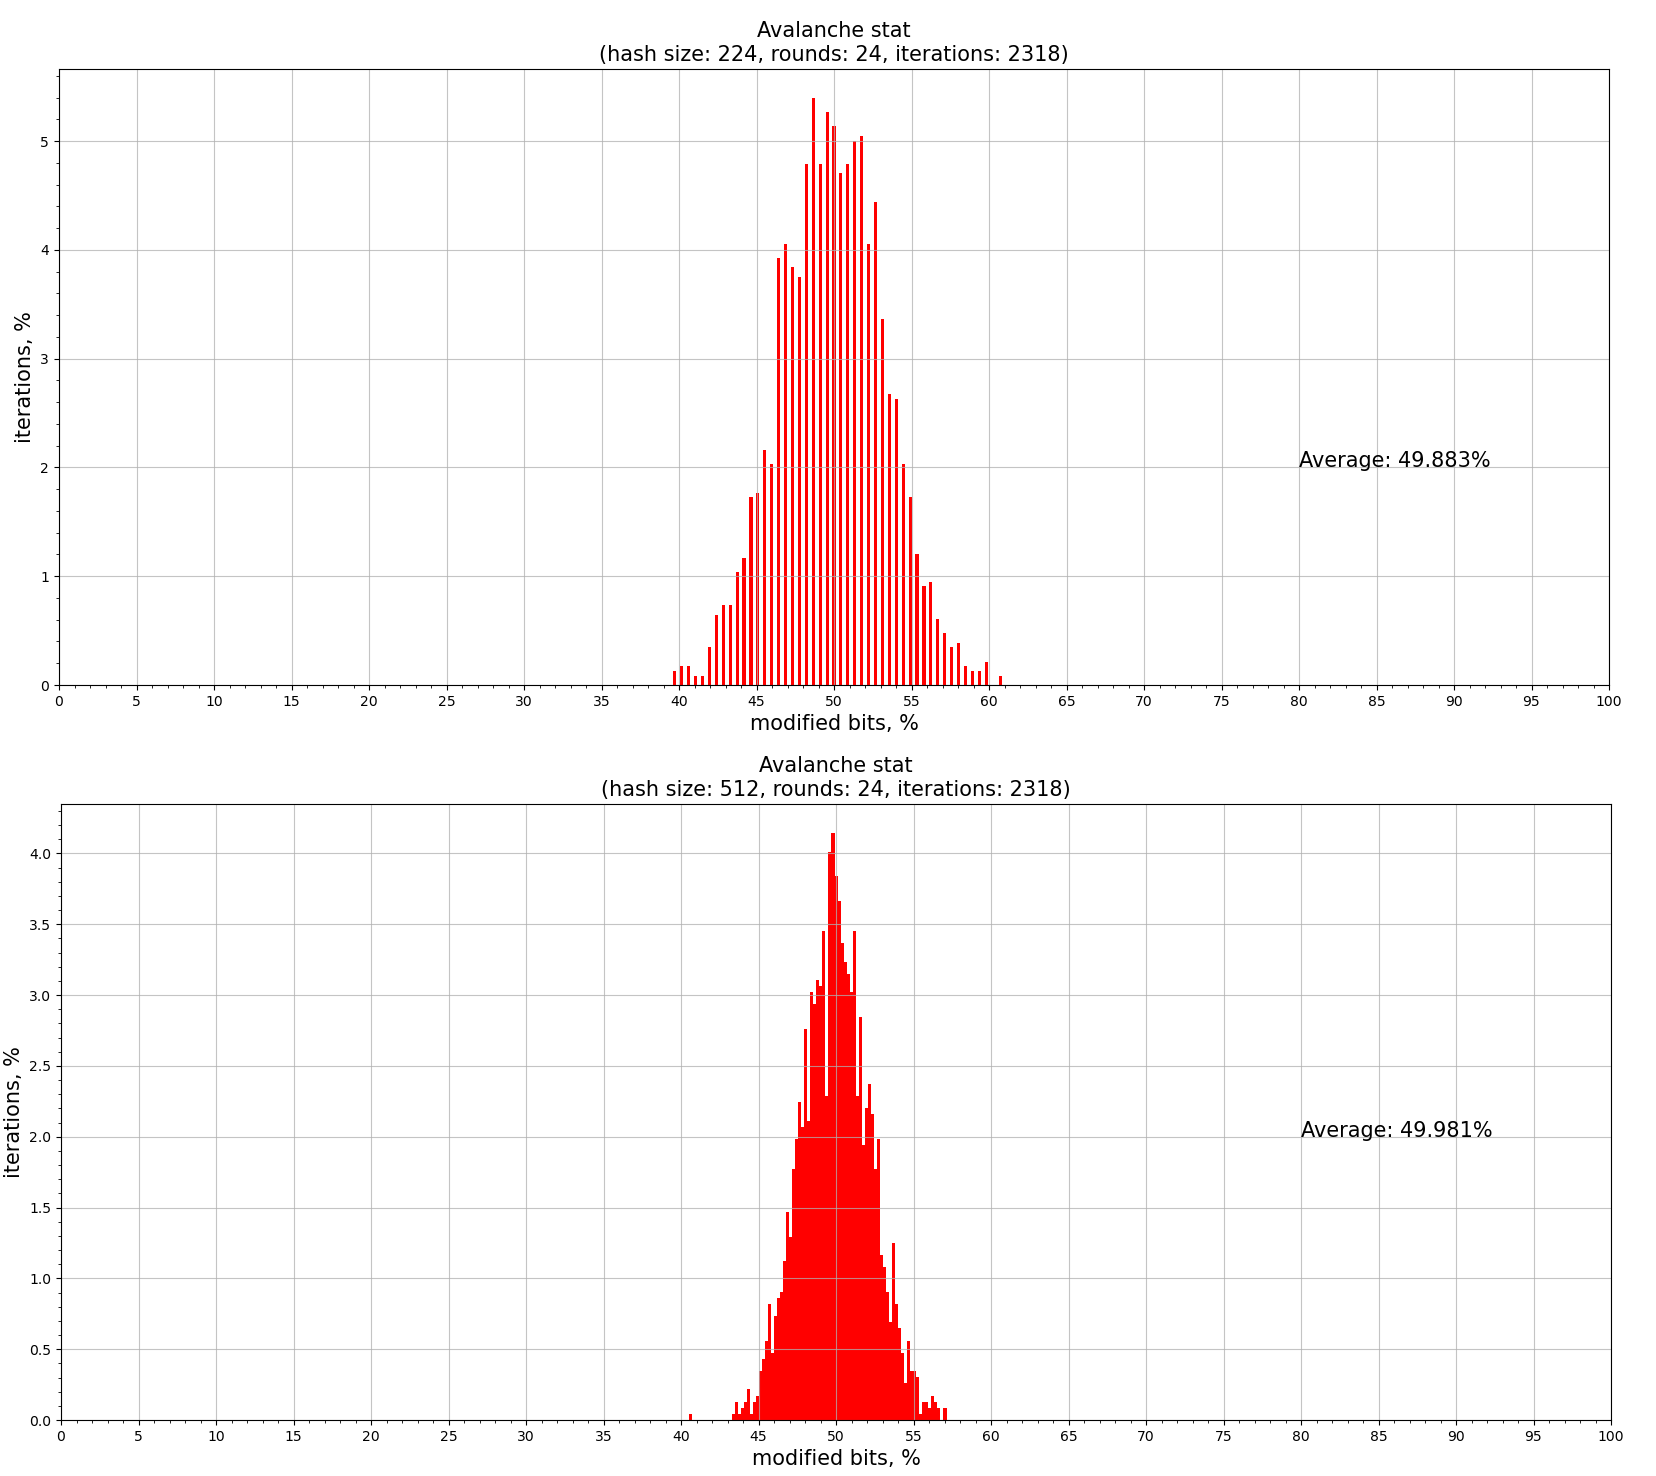
\includegraphics[width=180mm]{224-512_24.png}
	\caption{Хэш 224 бита с числом раундов 1, 2, 3 и 24}
\end{figure}	

	
	
	
	
\end{document} % конец документа